\subsection{Lab13: Recepción de señales de radio FM para Walkie-Talkie UHF}
%*********************
\begin{frame}{}

\pgfdeclareimage[width=\paperwidth,height=\paperheight]{bg}{imagenes/fondo_lab}
\setbeamertemplate{background}{\pgfuseimage{bg}}


\bfseries{\textrm{\LARGE Lab13 \newline\Large Recepción de señales\newline  de radio FM para \newline Walkie-Talkie UHF}}
\raggedright
\end{frame}
%*********************
\begin{frame}{Recepción de señales de radio FM para Walkie-Talkie UHF}

\pgfdeclareimage[width=\paperwidth,height=\paperheight]{bg}{imagenes/fondo3}
\setbeamertemplate{background}{\pgfuseimage{bg}}

\begin{figure}[H]
\centering
\vspace{-3mm}
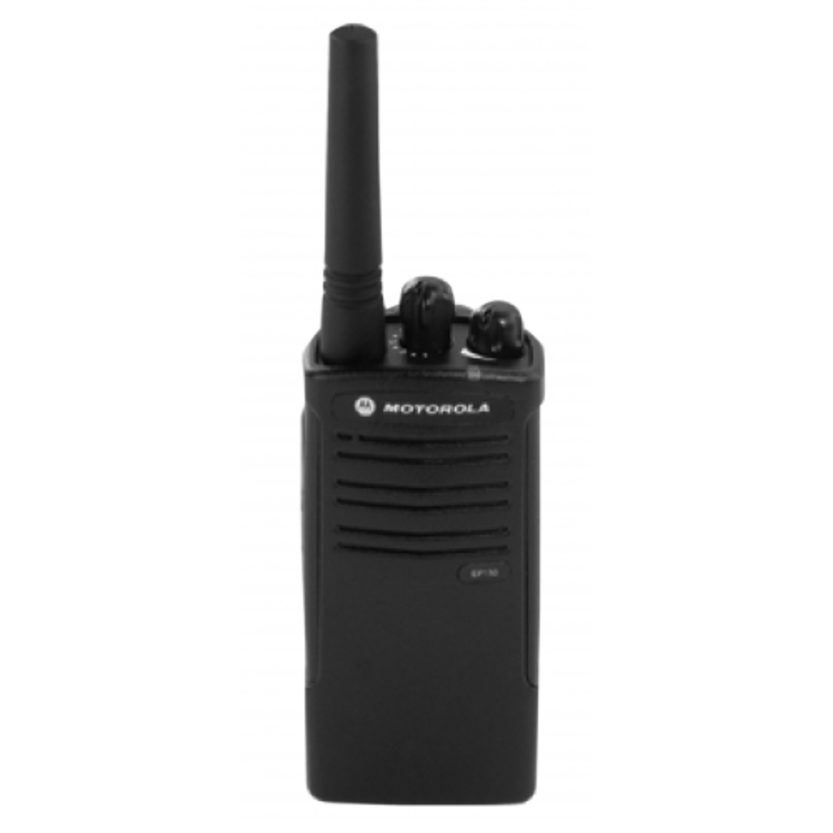
\includegraphics[width=\textwidth]{parte3/lab10/pdf/lab10_1.pdf}
\end{figure}

\end{frame}
%---------------------------------

\begin{frame}{Recepción de señales de radio FM para Walkie-Talkie UHF}


Para esta práctica se realiza el diagrama de bloques para captar las señales de las frecuencias portadoras de cada uno de los canales del radio EP150, a continuación se muestra el radio utilizado en esta práctica y su respectiva tabla de especificaciones, estas son necesarias durante la práctica, también se presenta el diagrama de bloques realizado para la captación de las portadoras.
    
\end{frame}
%---------------------------------

\begin{frame}{Especificaciones del radio}

Estas especificaciones serán necesarias con el fin de conocer el rango de frecuencia de operación del radio\cite{FichaTecnica}.

\begin{figure}[H]
\centering
\vspace{-3mm}
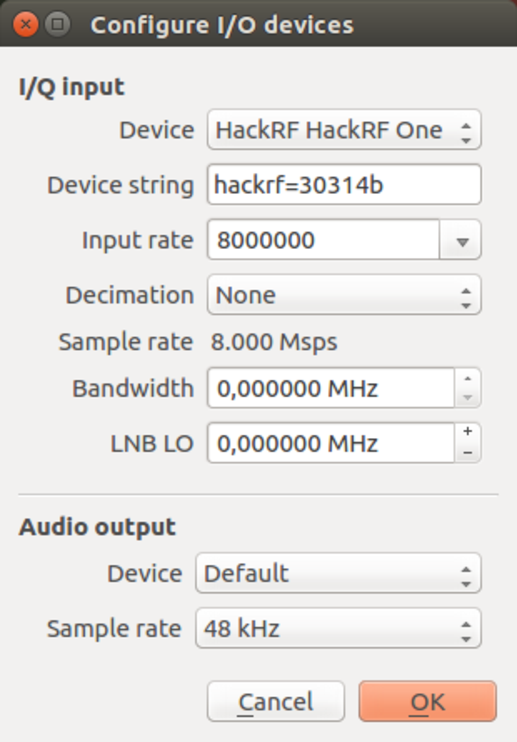
\includegraphics[width=\textwidth]{parte3/lab10/pdf/lab10_3.pdf}
\end{figure}

\end{frame}
%---------------------------------

\begin{frame}{GQRX}

Es necesario instalar el programa \texttt{gqrx}, útil para determinar las frecuencias de trabajo del radio en cada uno de sus canales, para instalarlo se usa:

\begin{block}{}
  \texttt{
  \ \ \ sudo apt-get update
    \begin{itemize}
      \item[] sudo apt-get install gqrx-sdr
    \end{itemize}}
\end{block}

\end{frame}
%---------------------------------

\begin{frame}{HackRF One}

Al iniciar el programa se configura el dispositivo, en este caso una Hack RF. Para verificar que esté conectada al PC se puede usar la orden:

\begin{block}{}
  \texttt{
  \ \ \ hackrf\_info}
\end{block}

\begin{figure}[H]
\centering
\vspace{-3mm}
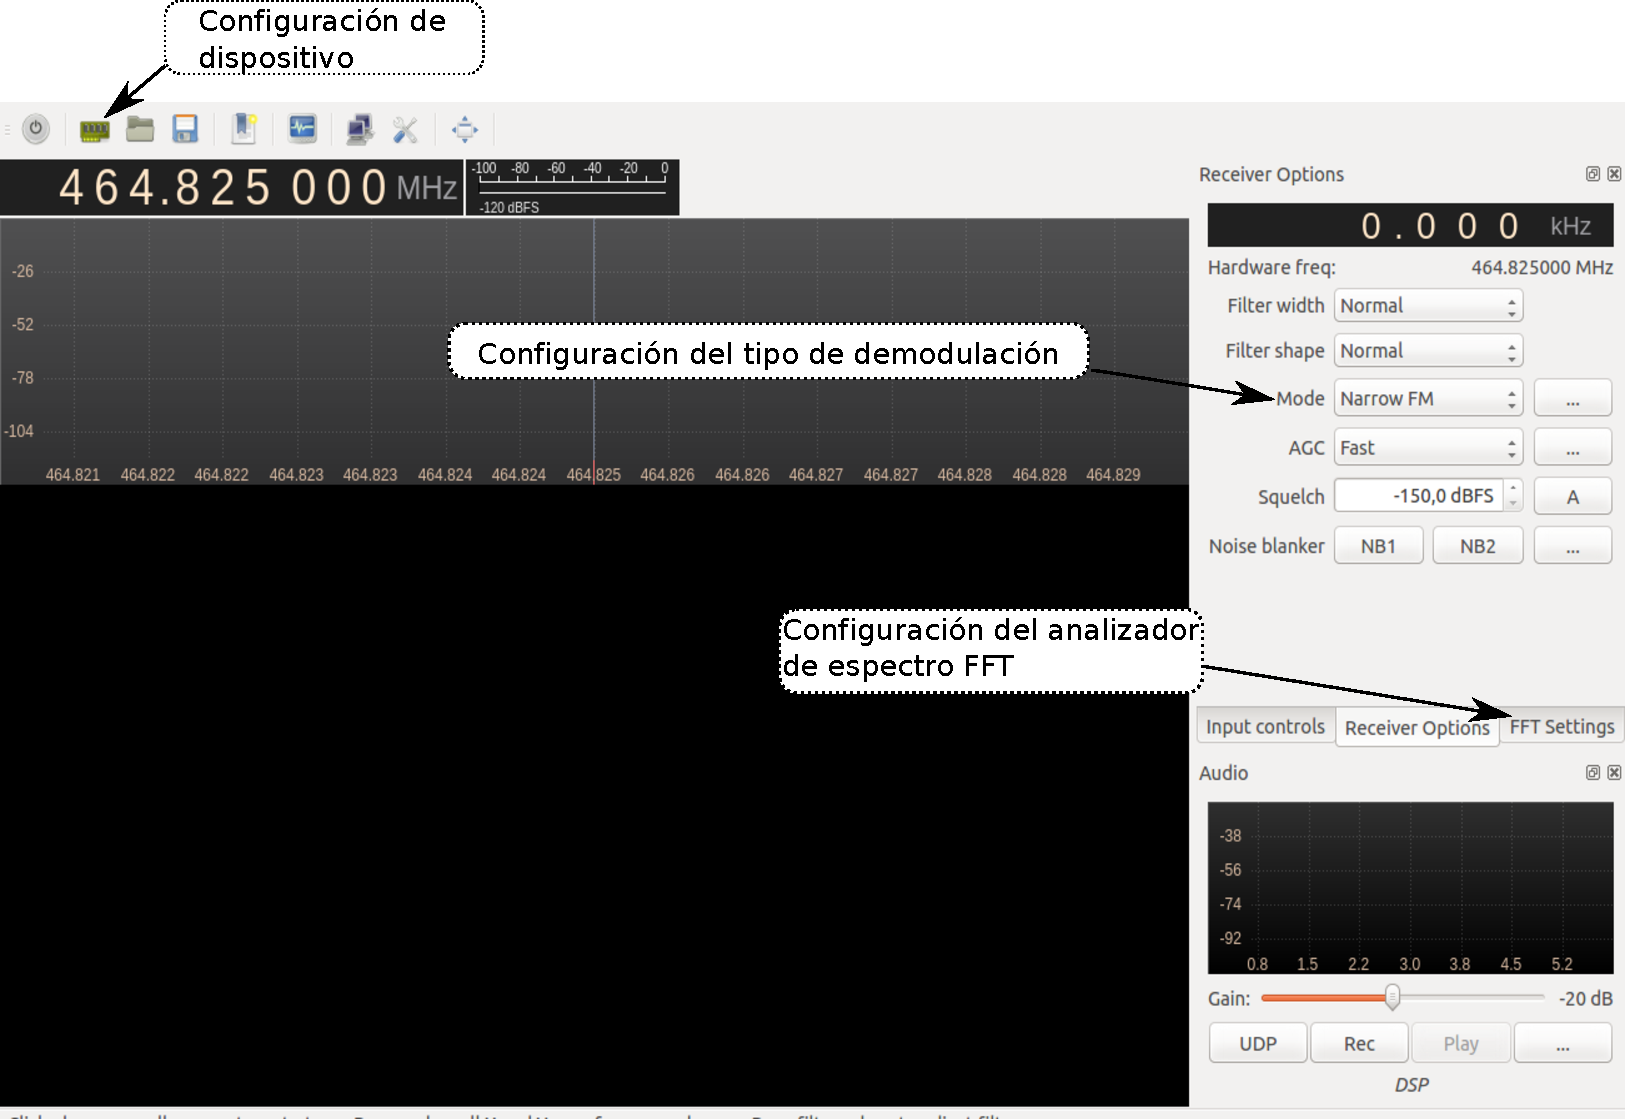
\includegraphics[width=.3\textwidth]{parte3/lab10/pdf/lab10_4.pdf}
\end{figure}

\end{frame}
%---------------------------------

\begin{frame}{Interfaz del programa}

\begin{figure}[H]
\centering
\vspace{-3mm}
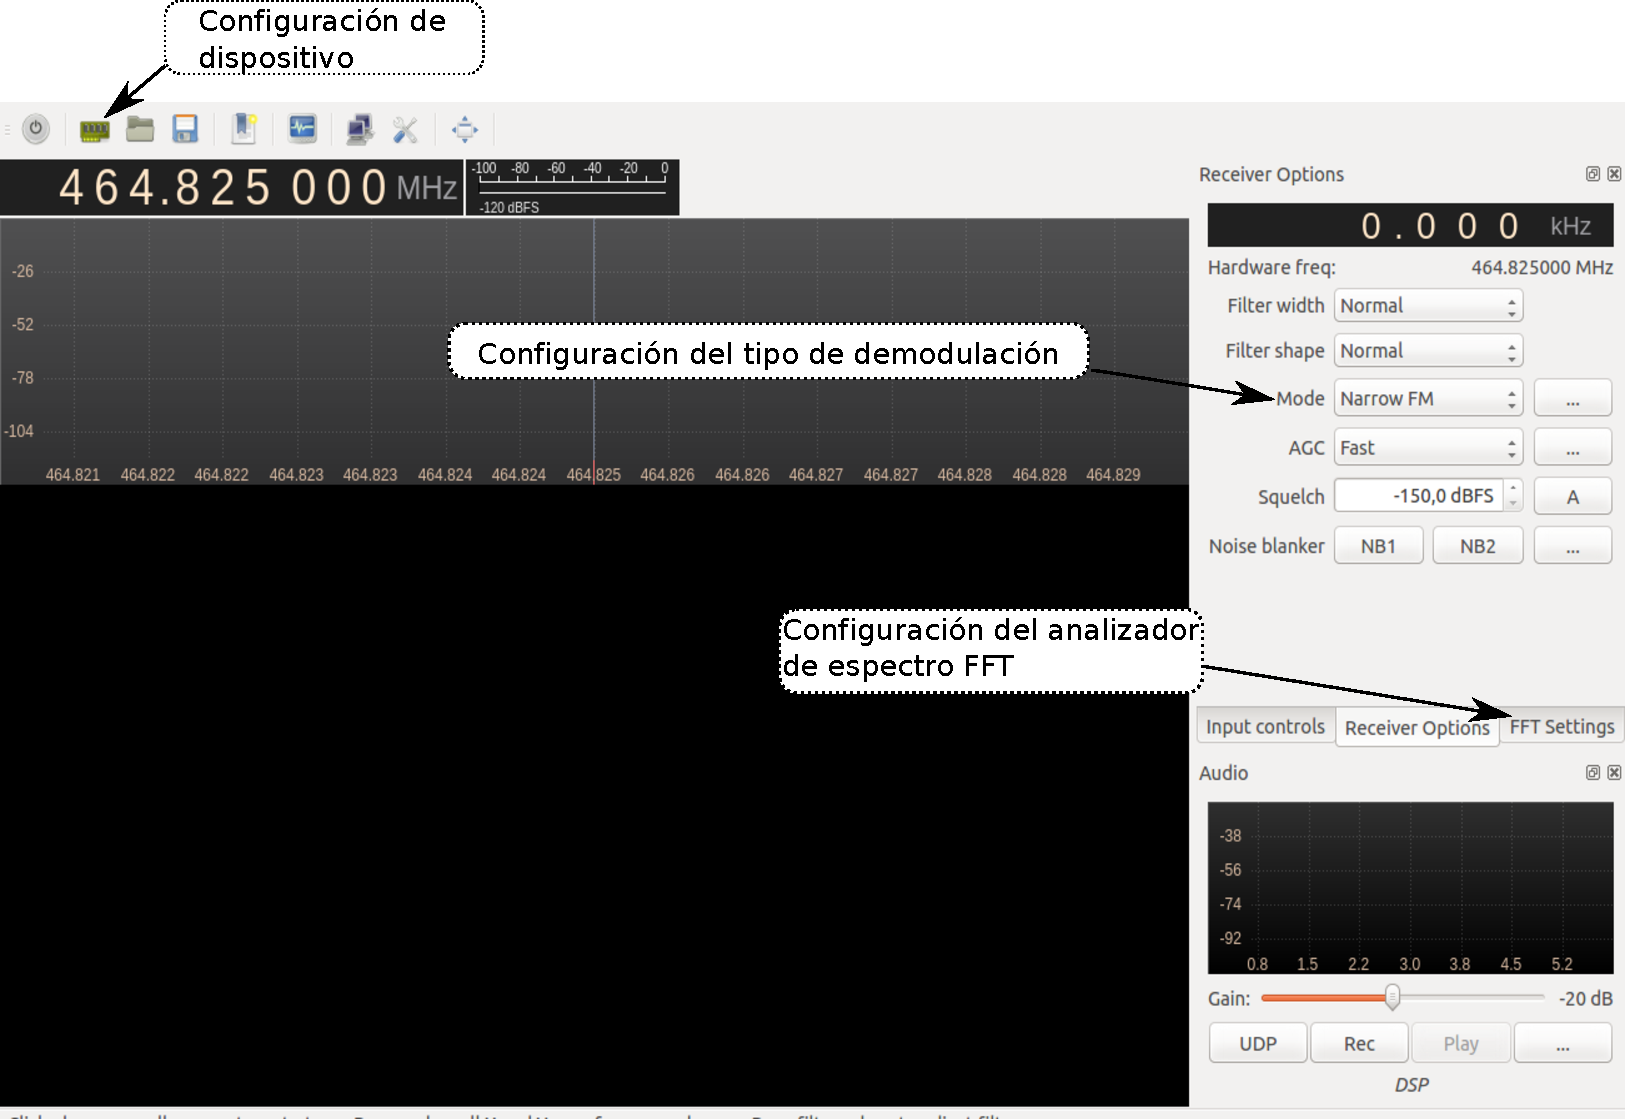
\includegraphics[width=.9\textwidth]{parte3/lab10/pdf/lab10_5.pdf}
\end{figure}

\end{frame}
%---------------------------------

\begin{frame}{Detectar frecuencias}

\begin{figure}[H]
\centering
\vspace{-3mm}
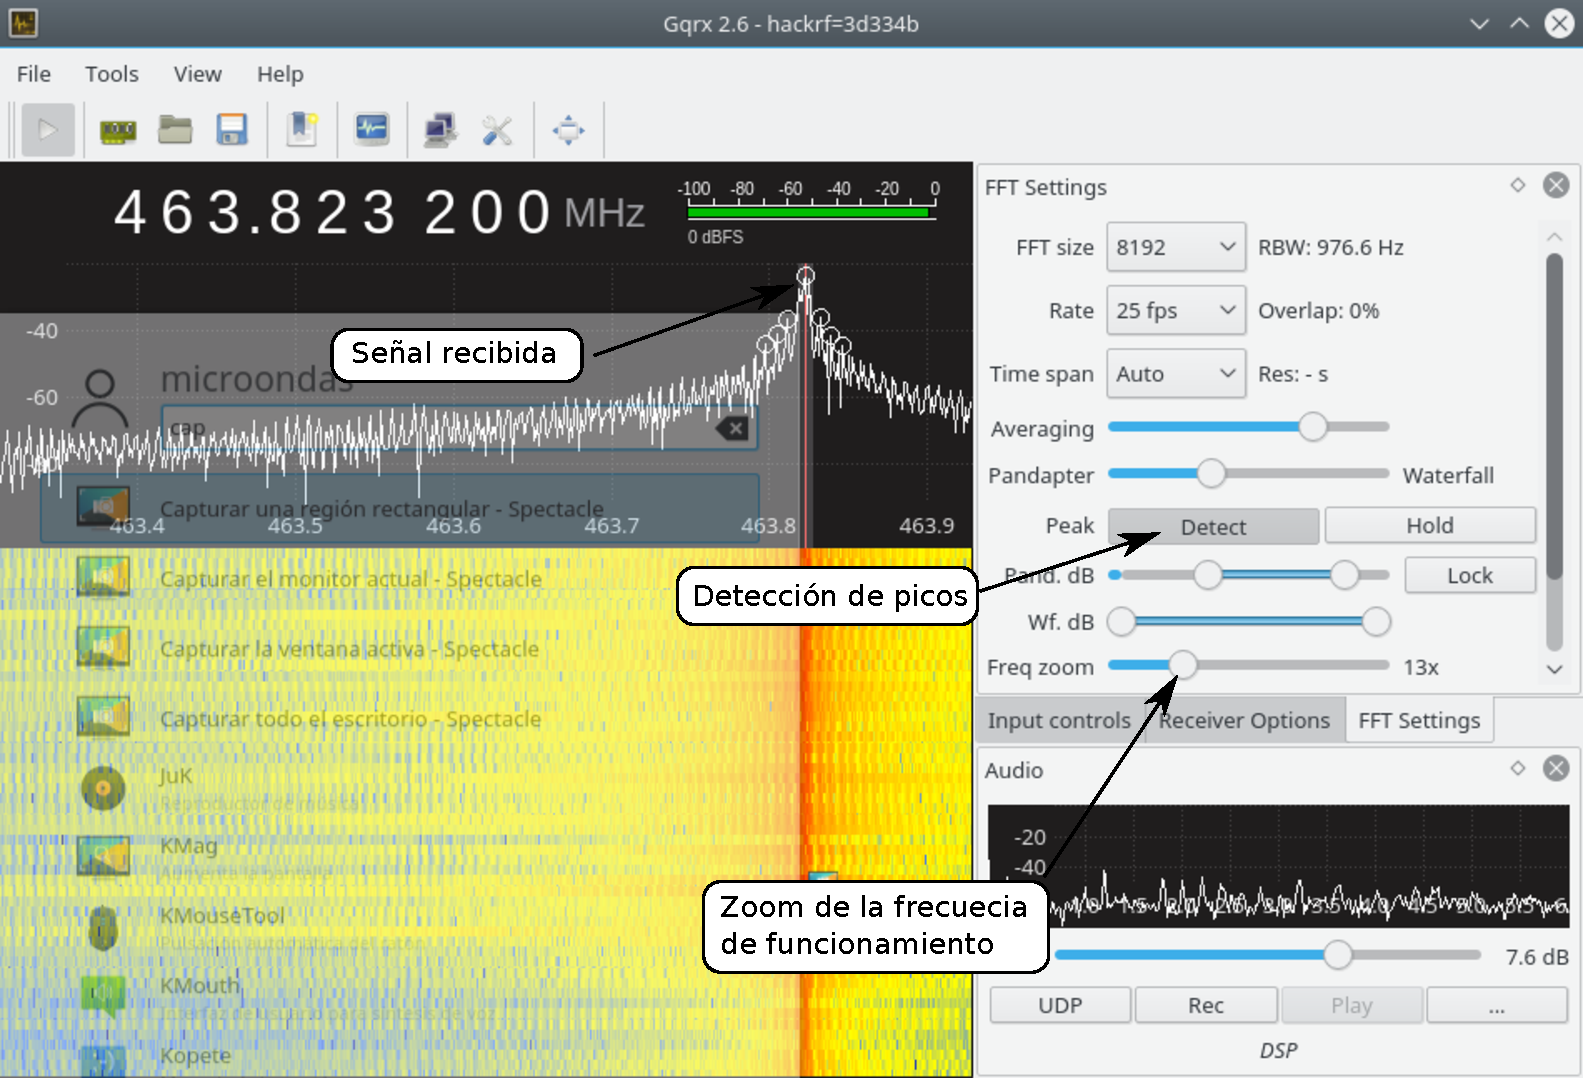
\includegraphics[width=\textwidth]{parte3/lab10/pdf/lab10_6.pdf}
\end{figure}

\end{frame}
%---------------------------------

\begin{frame}{Tabla de frecuencias}

Al variar los 8 canales disponibles del dispositivo, se logran encontrar las frecuencias correspondientes.


\begin{table}[]
\scriptsize
\centering
\begin{tabular}{|c|c|}
\hline

\rowcolor{BlueGreen!20}
\textbf{CANAL} & \textbf{FRECUENCIA DE SEÑAL PORTADORA} \\ \hline
1              & 462,5750 MHz                           \\ \hline
2              & 462,6250 MHz                           \\ \hline
3              & 462,6750 MHz                           \\ \hline
4              & 463,5500 MHz                           \\ \hline
5              & 463,6250 MHz                           \\ \hline
6              & 463,7625 MHz                           \\ \hline
7              & 463,7750 MHz                           \\ \hline
8              & 463,8250 MHz                           \\ \hline
\end{tabular}
\end{table}

\end{frame}
%---------------------------------

\begin{frame}{}

Obtenidos los rangos de frecuencias de cada uno de los canales del radio, se realiza el diagrama de bloques con el fin de observar las señales portadoras de cada uno de los canales en un osciloscopio.

\begin{figure}[H]
\centering
\vspace{-3mm}
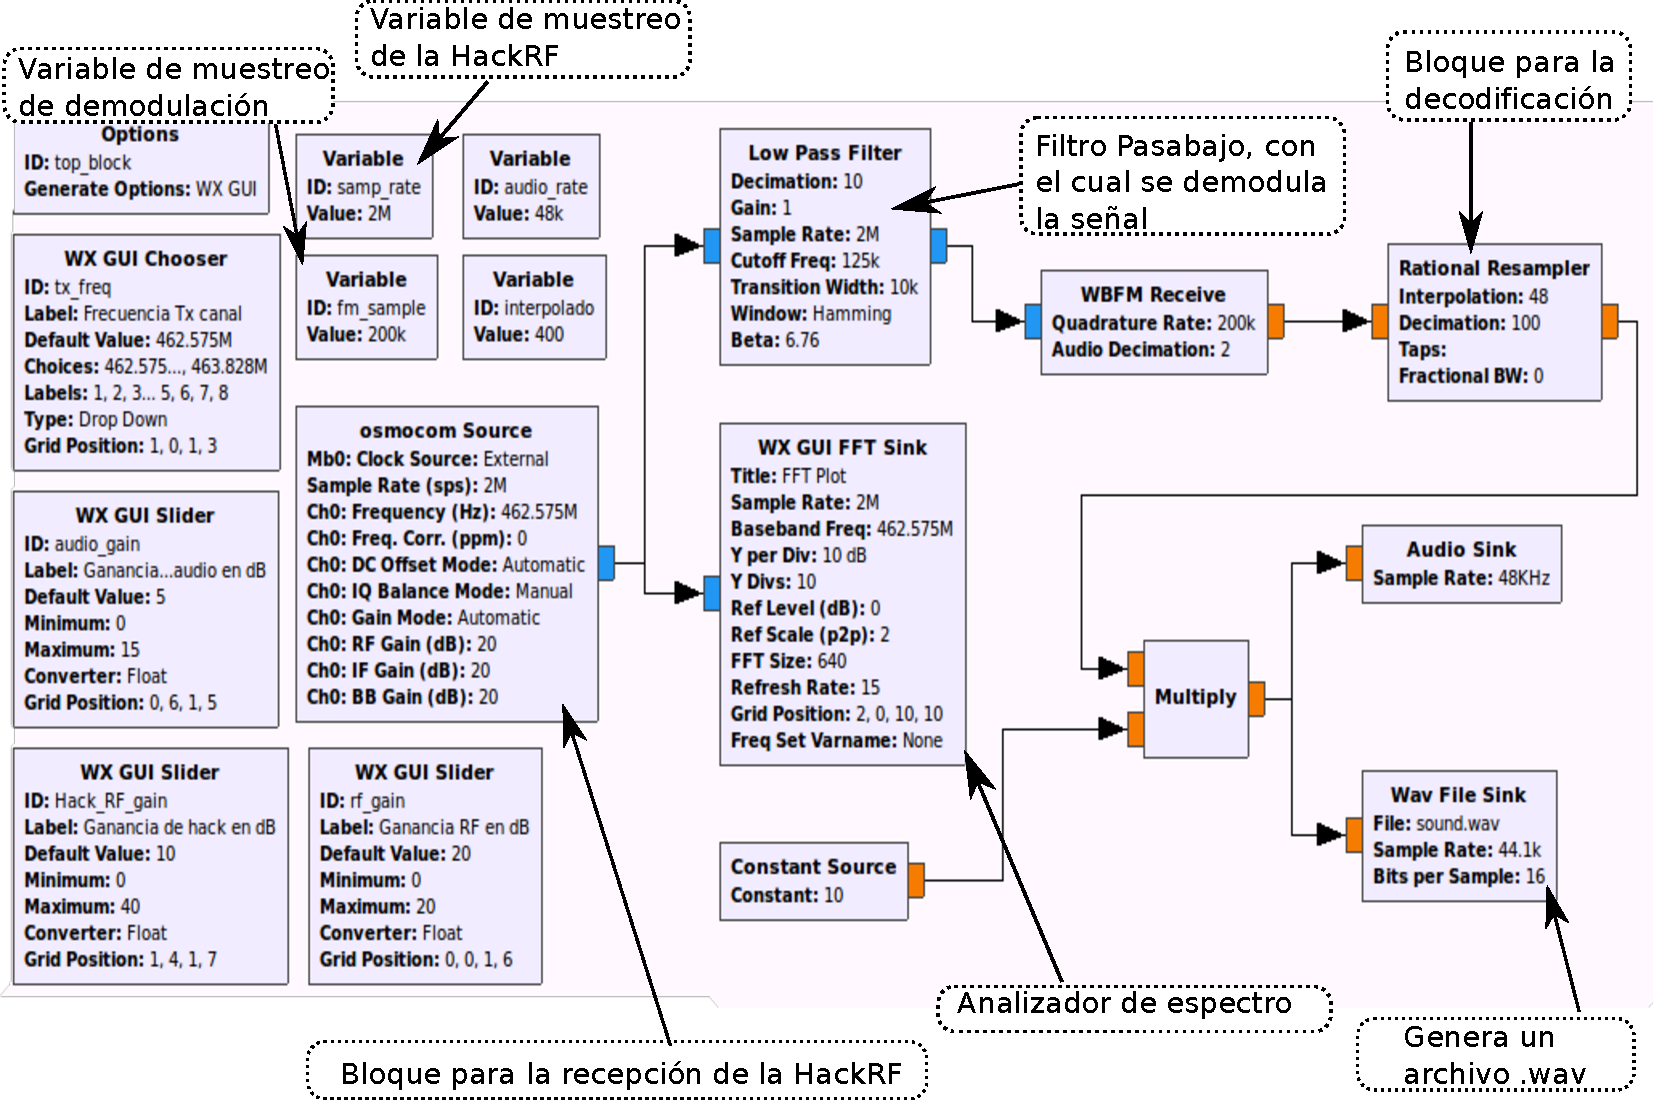
\includegraphics[width=.9\textwidth]{parte3/lab10/pdf/lab10_8.pdf}
\end{figure}

\end{frame}
%---------------------------------

\begin{frame}{Configuraciones}

Se configura el bloque con el que se recibe la señal con la tarjeta HackRF donde nos permite configurar más de una tarjeta en la misma conexión.

\begin{figure}[H]
\centering
\vspace{-3mm}
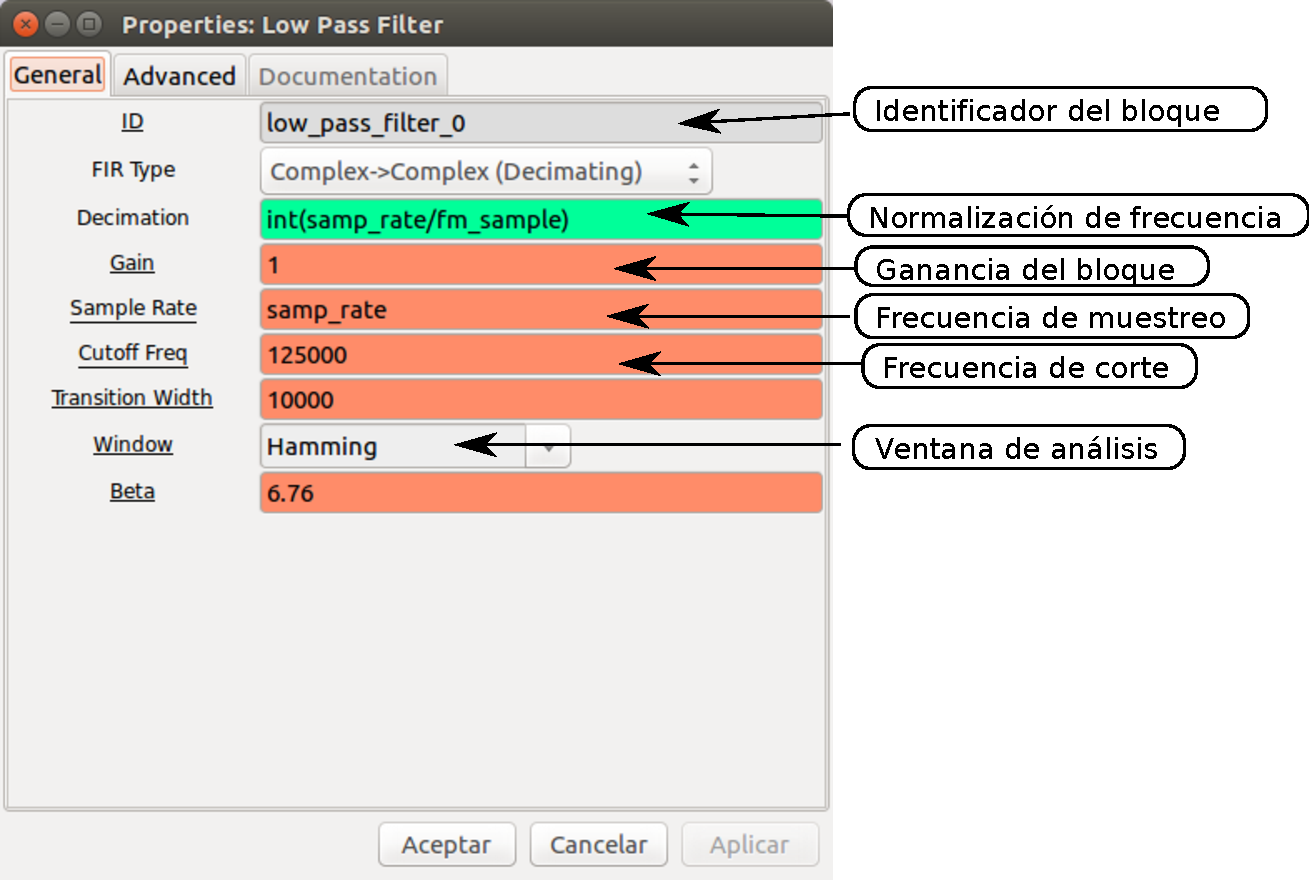
\includegraphics[width=.8\textwidth]{parte3/lab10/pdf/lab10_9.pdf}
\end{figure}

\end{frame}
%---------------------------------

\begin{frame}{Configuraciones}

Se configura el bloque con el que se demodula la señal con la tarjeta HackRF.

\begin{figure}[H]
\centering
\vspace{-3mm}
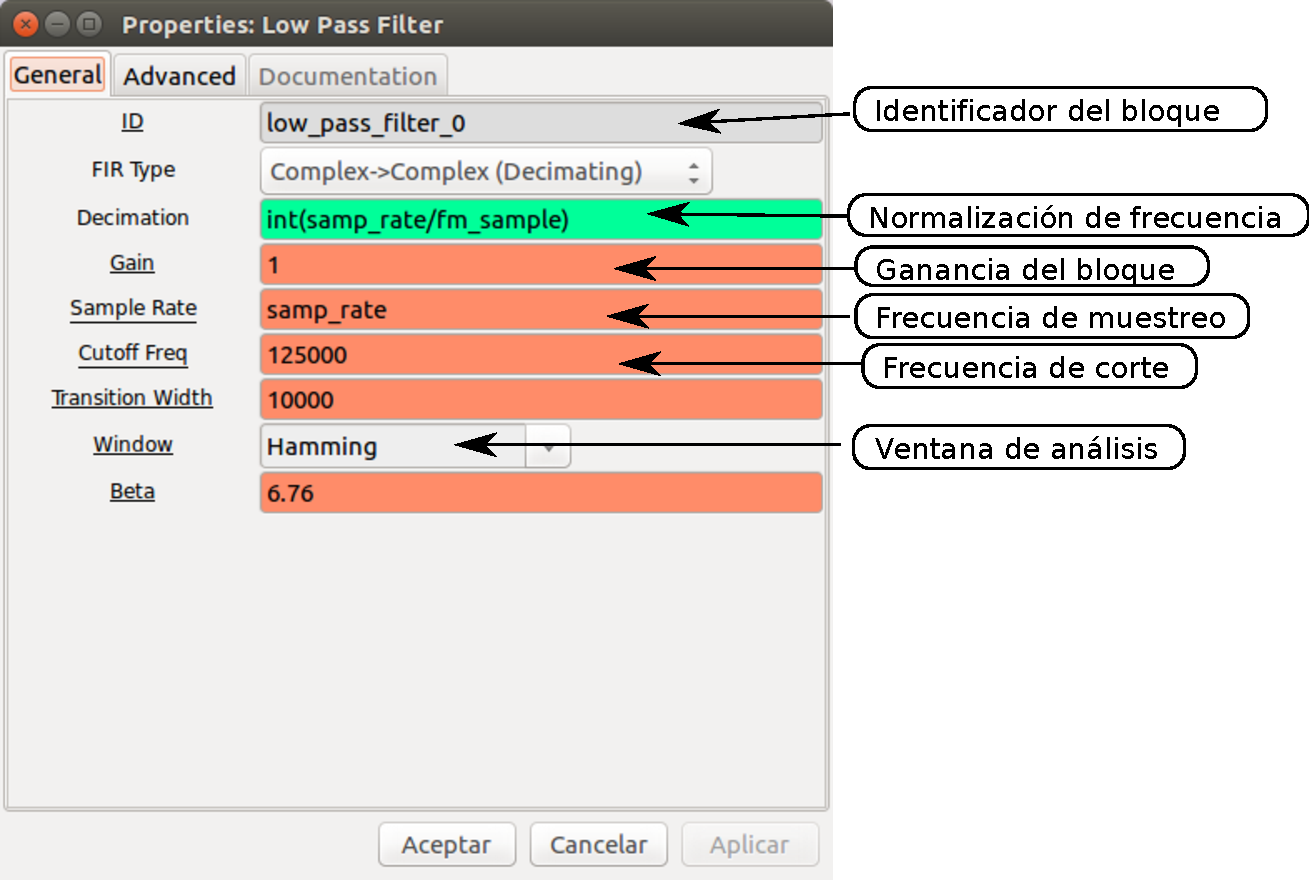
\includegraphics[width=.8\textwidth]{parte3/lab10/pdf/lab10_10.pdf}
\end{figure}

\end{frame}
%---------------------------------

\begin{frame}{Configuraciones}

Se configura el bloque con el cual se decodifica la información mediante una comparación de frecuencias:

\begin{figure}[H]
\centering
\vspace{-3mm}
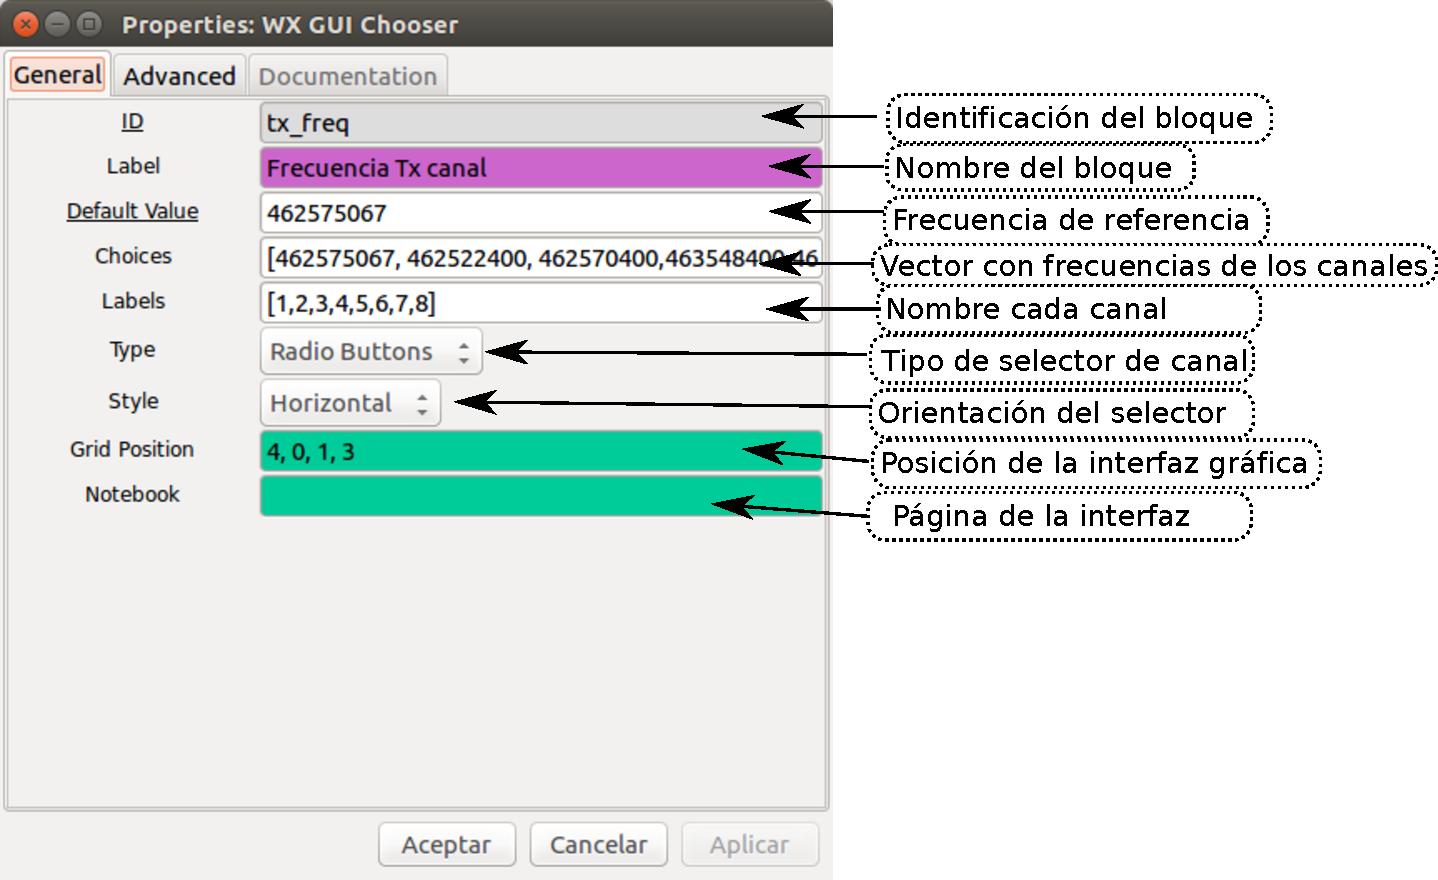
\includegraphics[width=.5\textwidth]{parte3/lab10/pdf/lab10_11.pdf}
\end{figure}

\end{frame}
%---------------------------------

\begin{frame}{Configuraciones}

Se configura el bloque que se utiliza como el selector de canal:

\begin{figure}[H]
\centering
\vspace{-3mm}
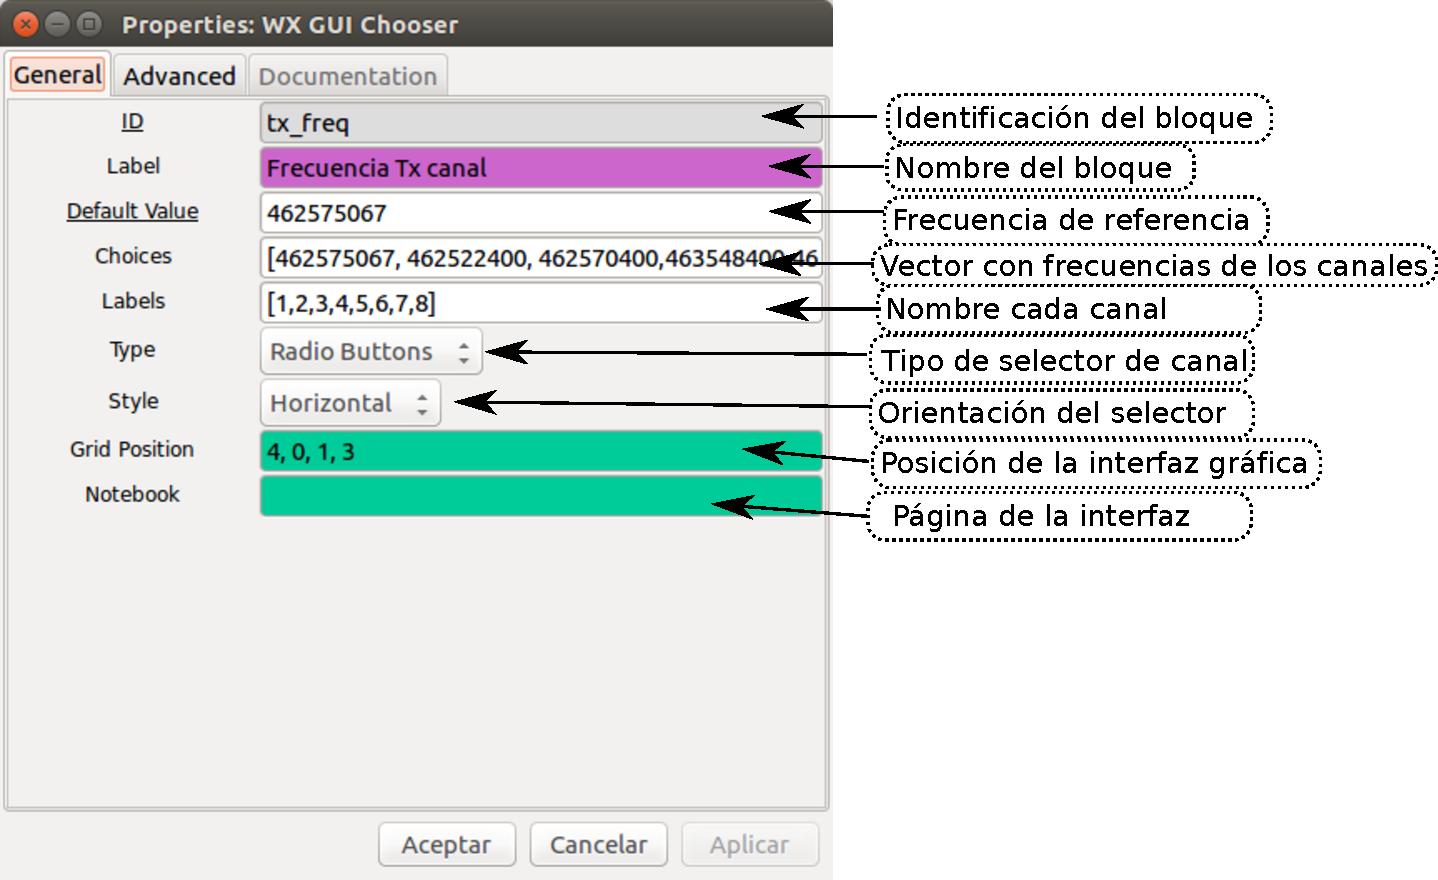
\includegraphics[width=\textwidth]{parte3/lab10/pdf/lab10_12.pdf}
\end{figure}

\end{frame}
%---------------------------------

\begin{frame}{Interfaz gráfica para la demodulación de la señal}

\begin{figure}[H]
\centering
\vspace{-3mm}
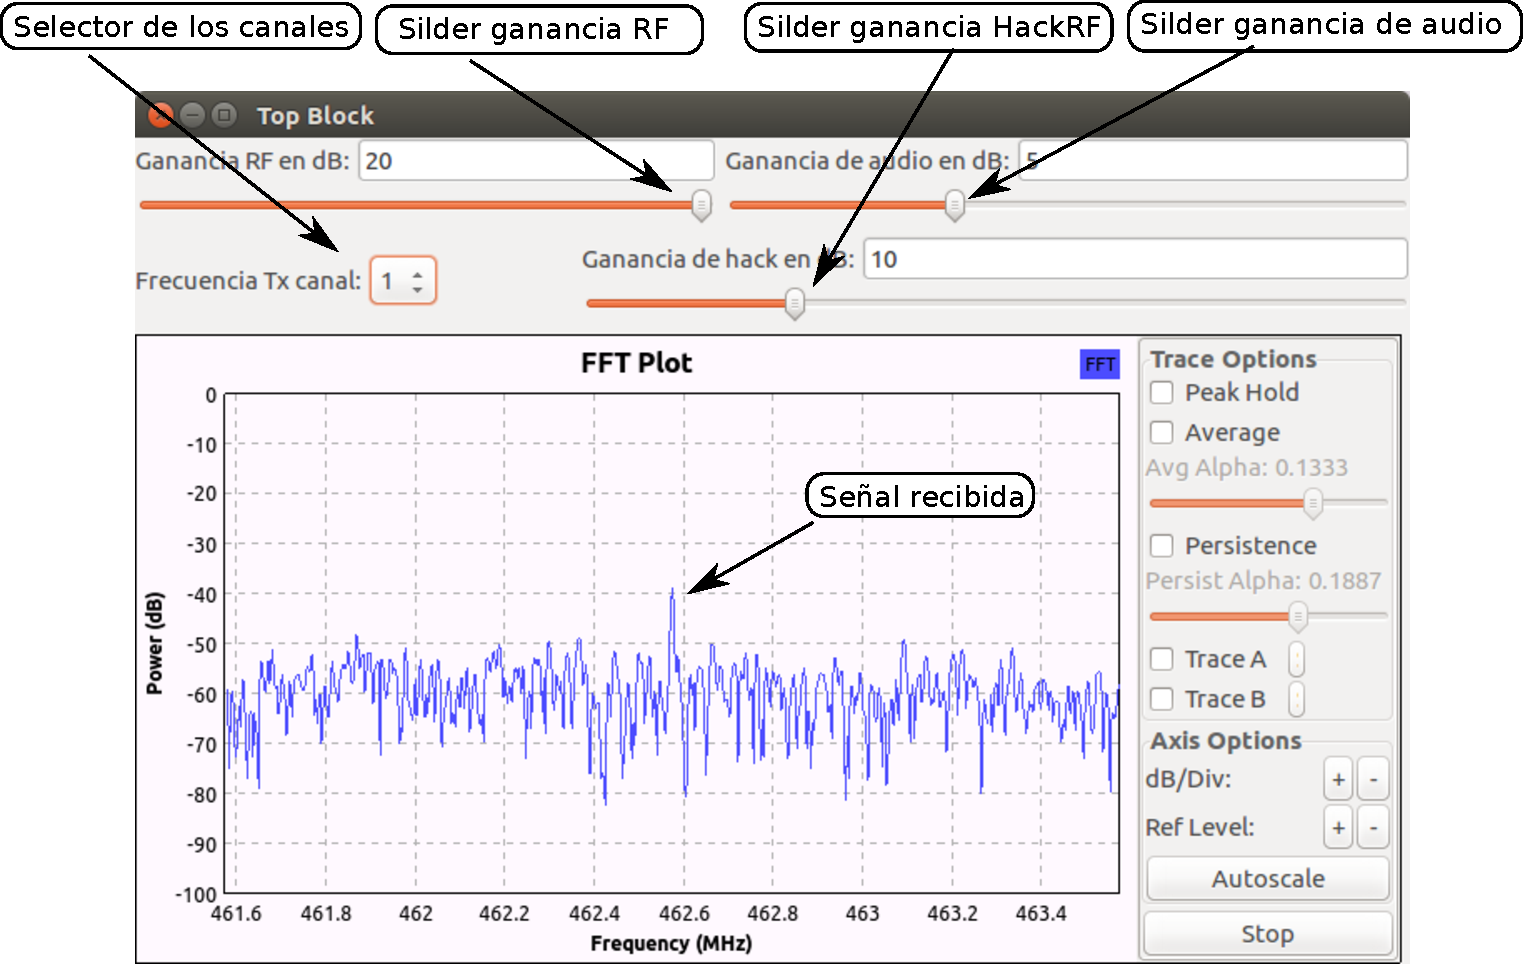
\includegraphics[width=\textwidth]{parte3/lab10/pdf/lab10_13.pdf}
\end{figure}

\end{frame}
%---------------------------------

\begin{frame}{Conclusión}

Se observa y escucha la señal recibida por el EP150 y eventualmente la señal que envía una Hack RF transmisora de FM. El tiempo que corre el programa y esta la interfaz abierta graba y deposita la información en un WAV.

\end{frame}
%---------------------------------

